% Options for packages loaded elsewhere
\PassOptionsToPackage{unicode}{hyperref}
\PassOptionsToPackage{hyphens}{url}
%
\documentclass[
]{article}
\usepackage{amsmath,amssymb}
\usepackage{lmodern}
\usepackage{iftex}
\ifPDFTeX
  \usepackage[T1]{fontenc}
  \usepackage[utf8]{inputenc}
  \usepackage{textcomp} % provide euro and other symbols
\else % if luatex or xetex
  \usepackage{unicode-math}
  \defaultfontfeatures{Scale=MatchLowercase}
  \defaultfontfeatures[\rmfamily]{Ligatures=TeX,Scale=1}
\fi
% Use upquote if available, for straight quotes in verbatim environments
\IfFileExists{upquote.sty}{\usepackage{upquote}}{}
\IfFileExists{microtype.sty}{% use microtype if available
  \usepackage[]{microtype}
  \UseMicrotypeSet[protrusion]{basicmath} % disable protrusion for tt fonts
}{}
\makeatletter
\@ifundefined{KOMAClassName}{% if non-KOMA class
  \IfFileExists{parskip.sty}{%
    \usepackage{parskip}
  }{% else
    \setlength{\parindent}{0pt}
    \setlength{\parskip}{6pt plus 2pt minus 1pt}}
}{% if KOMA class
  \KOMAoptions{parskip=half}}
\makeatother
\usepackage{xcolor}
\usepackage[margin=1in]{geometry}
\usepackage{graphicx}
\makeatletter
\def\maxwidth{\ifdim\Gin@nat@width>\linewidth\linewidth\else\Gin@nat@width\fi}
\def\maxheight{\ifdim\Gin@nat@height>\textheight\textheight\else\Gin@nat@height\fi}
\makeatother
% Scale images if necessary, so that they will not overflow the page
% margins by default, and it is still possible to overwrite the defaults
% using explicit options in \includegraphics[width, height, ...]{}
\setkeys{Gin}{width=\maxwidth,height=\maxheight,keepaspectratio}
% Set default figure placement to htbp
\makeatletter
\def\fps@figure{htbp}
\makeatother
\setlength{\emergencystretch}{3em} % prevent overfull lines
\providecommand{\tightlist}{%
  \setlength{\itemsep}{0pt}\setlength{\parskip}{0pt}}
\setcounter{secnumdepth}{-\maxdimen} % remove section numbering
\ifLuaTeX
  \usepackage{selnolig}  % disable illegal ligatures
\fi
\IfFileExists{bookmark.sty}{\usepackage{bookmark}}{\usepackage{hyperref}}
\IfFileExists{xurl.sty}{\usepackage{xurl}}{} % add URL line breaks if available
\urlstyle{same} % disable monospaced font for URLs
\hypersetup{
  pdftitle={Evaluating the breeding potential of cultivated lentils for protein and amino acid concentration and quality},
  pdfauthor={Derek Michael Wright derek.wright@usask.ca},
  hidelinks,
  pdfcreator={LaTeX via pandoc}}

\title{Evaluating the breeding potential of cultivated lentils for
protein and amino acid concentration and quality}
\usepackage{etoolbox}
\makeatletter
\providecommand{\subtitle}[1]{% add subtitle to \maketitle
  \apptocmd{\@title}{\par {\large #1 \par}}{}{}
}
\makeatother
\subtitle{\emph{unpublished}}
\author{Derek Michael Wright
\href{mailto:derek.wright@usask.ca}{\nolinkurl{derek.wright@usask.ca}}}
\date{10-11-2023}

\begin{document}
\maketitle

{
\setcounter{tocdepth}{2}
\tableofcontents
}
\pagebreak

\begin{center}\rule{0.5\linewidth}{0.5pt}\end{center}

\href{https://github.com/derekmichaelwright/AGILE_LDP_Protein}{Derek
Wright, Jiayi Hang, James D House \& Kirstin E Bett (2020)
\textbf{Lentil Protein}. \emph{unpublished}}

which is follow-up to:

\begin{quote}
\begin{itemize}
\tightlist
\item
  \href{https://doi.org/10.1016/j.lwt.2022.113669}{Jiayi Hang, Da Shi,
  Jason Neufeld, Kirstin E. Bett \& James D. House. \textbf{Prediction
  of protein and amino acid concentration in whole and ground lentils
  using near-infrared reflectance spectroscopy}. \emph{LWT}.
  (\textbf{2022}) 165: 113669. doi.org/10.1016/j.lwt.2022.113669}
\end{itemize}
\end{quote}

\&

\begin{quote}
\begin{itemize}
\tightlist
\item
  \href{https://doi.org/10.1002/ppp3.10158}{Derek M. Wright, Sandesh
  Neupane, Taryn Heidecker, Teketel A. Haile, Crystal Chan, Clarice J.
  Coyne, Rebecca J. McGee, Sripada Udupa, Fatima Henkrar, Eleonora
  Barilli, Diego Rubiales, Tania Gioia, Giuseppina Logozzo, Stefania
  Marzario, Reena Mehra, Ashutosh Sarker, Rajeev Dhakal, Babul Anwar,
  Debashish Sarker, Albert Vandenberg \& Kirstin E. Bett.
  \textbf{Understanding photothermal interactions can help expand
  production range and increase genetic diversity of lentil (\emph{Lens
  culinaris} Medik.)}. \emph{Plants, People, Planet}. (\textbf{2020})
  3(2): 171-181. doi.org/10.1002/ppp3.10158}
\end{itemize}
\end{quote}

\begin{center}\rule{0.5\linewidth}{0.5pt}\end{center}

\begin{quote}
\begin{itemize}
\tightlist
\item
  \url{https://github.com/derekmichaelwright/AGILE_LDP_Protein}
\item
  \href{https://github.com/derekmichaelwright/AGILE_LDP_Protein/raw/master/README.pdf}{View
  as pdf}
\item
  \href{https://derekmichaelwright.github.io/AGILE_LDP_Protein/README.html}{View
  as HTML}
\item
  \href{https://derekmichaelwright.github.io/AGILE_LDP_Protein/LDP_Protein_Vignette.html}{Source
  Code Vignette (LDP\_Protein\_Vignette.html)}
\end{itemize}
\end{quote}

\hypertarget{contents}{%
\section{Contents}\label{contents}}

\begin{itemize}
\tightlist
\item
  \protect\hyperlink{figures}{Figures}
\item
  \protect\hyperlink{supplemental-figures}{Supplemental Figures}
\item
  \protect\hyperlink{additional-figures}{Additional Figures}
\end{itemize}

\hypertarget{agile}{%
\section{AGILE}\label{agile}}

\includegraphics[width=0.75\textwidth,height=\textheight]{Additional/img_Agile.png}

\pagebreak

\hypertarget{collaborators}{%
\subsection{Collaborators}\label{collaborators}}

\begin{itemize}
\tightlist
\item
  Department of Plant Sciences and Crop Development Centre, University
  of Saskatchewan, Saskatoon, Saskatchewan, Canada
\item
  Department of Food and Human Nutritional Sciences, Faculty of
  Agriculture and Food Science, University of Manitoba, Winnipeg, MB,
  Canada
\end{itemize}

\begin{center}\rule{0.5\linewidth}{0.5pt}\end{center}

\hypertarget{supplemental-table-1}{%
\section{Supplemental Table 1}\label{supplemental-table-1}}

\url{Supplemental_table_01.csv}

\begin{center}\rule{0.5\linewidth}{0.5pt}\end{center}

\hypertarget{figures}{%
\section{Figures}\label{figures}}

\hypertarget{figure-1}{%
\subsection{Figure 1}\label{figure-1}}

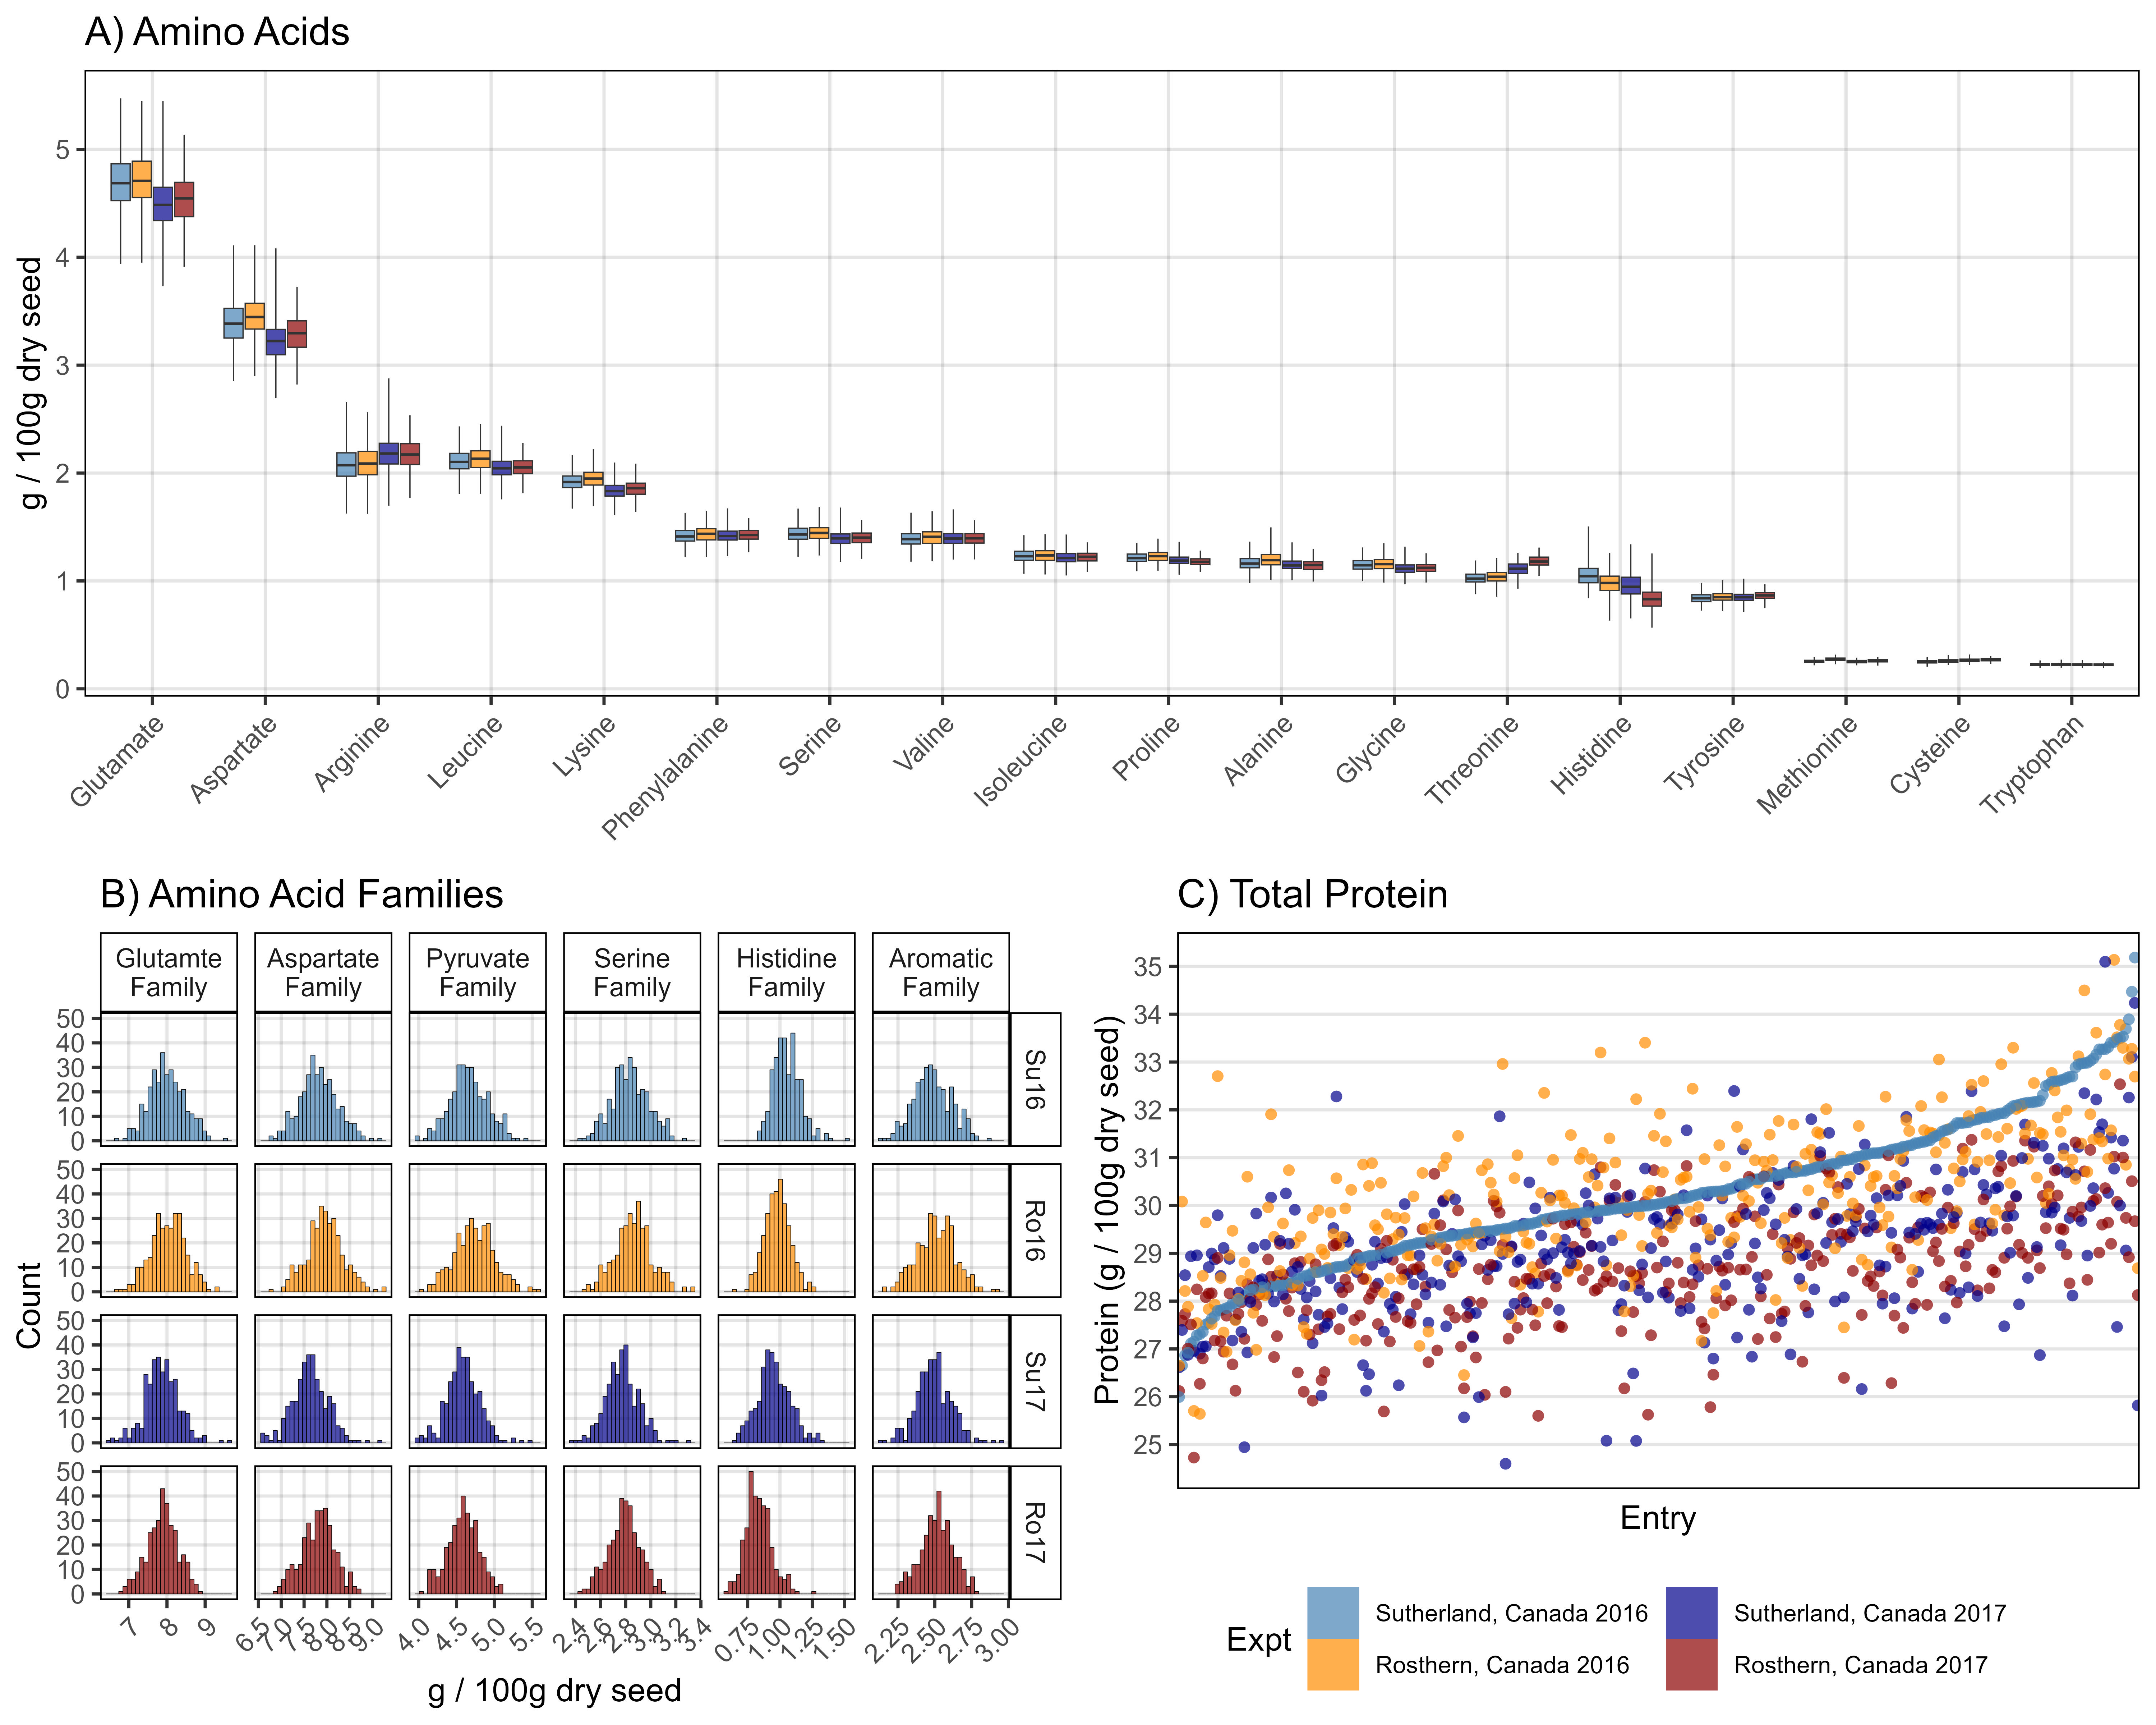
\includegraphics{Figure_01.jpg}

\begin{center}\rule{0.5\linewidth}{0.5pt}\end{center}

\hypertarget{figure-2}{%
\subsection{Figure 2}\label{figure-2}}

\includegraphics{Figure_02.jpg}

\begin{center}\rule{0.5\linewidth}{0.5pt}\end{center}

\hypertarget{figure-3}{%
\subsection{Figure 3}\label{figure-3}}

\includegraphics{Figure_03.jpg}

\begin{center}\rule{0.5\linewidth}{0.5pt}\end{center}

\hypertarget{figure-4}{%
\subsection{Figure 4}\label{figure-4}}

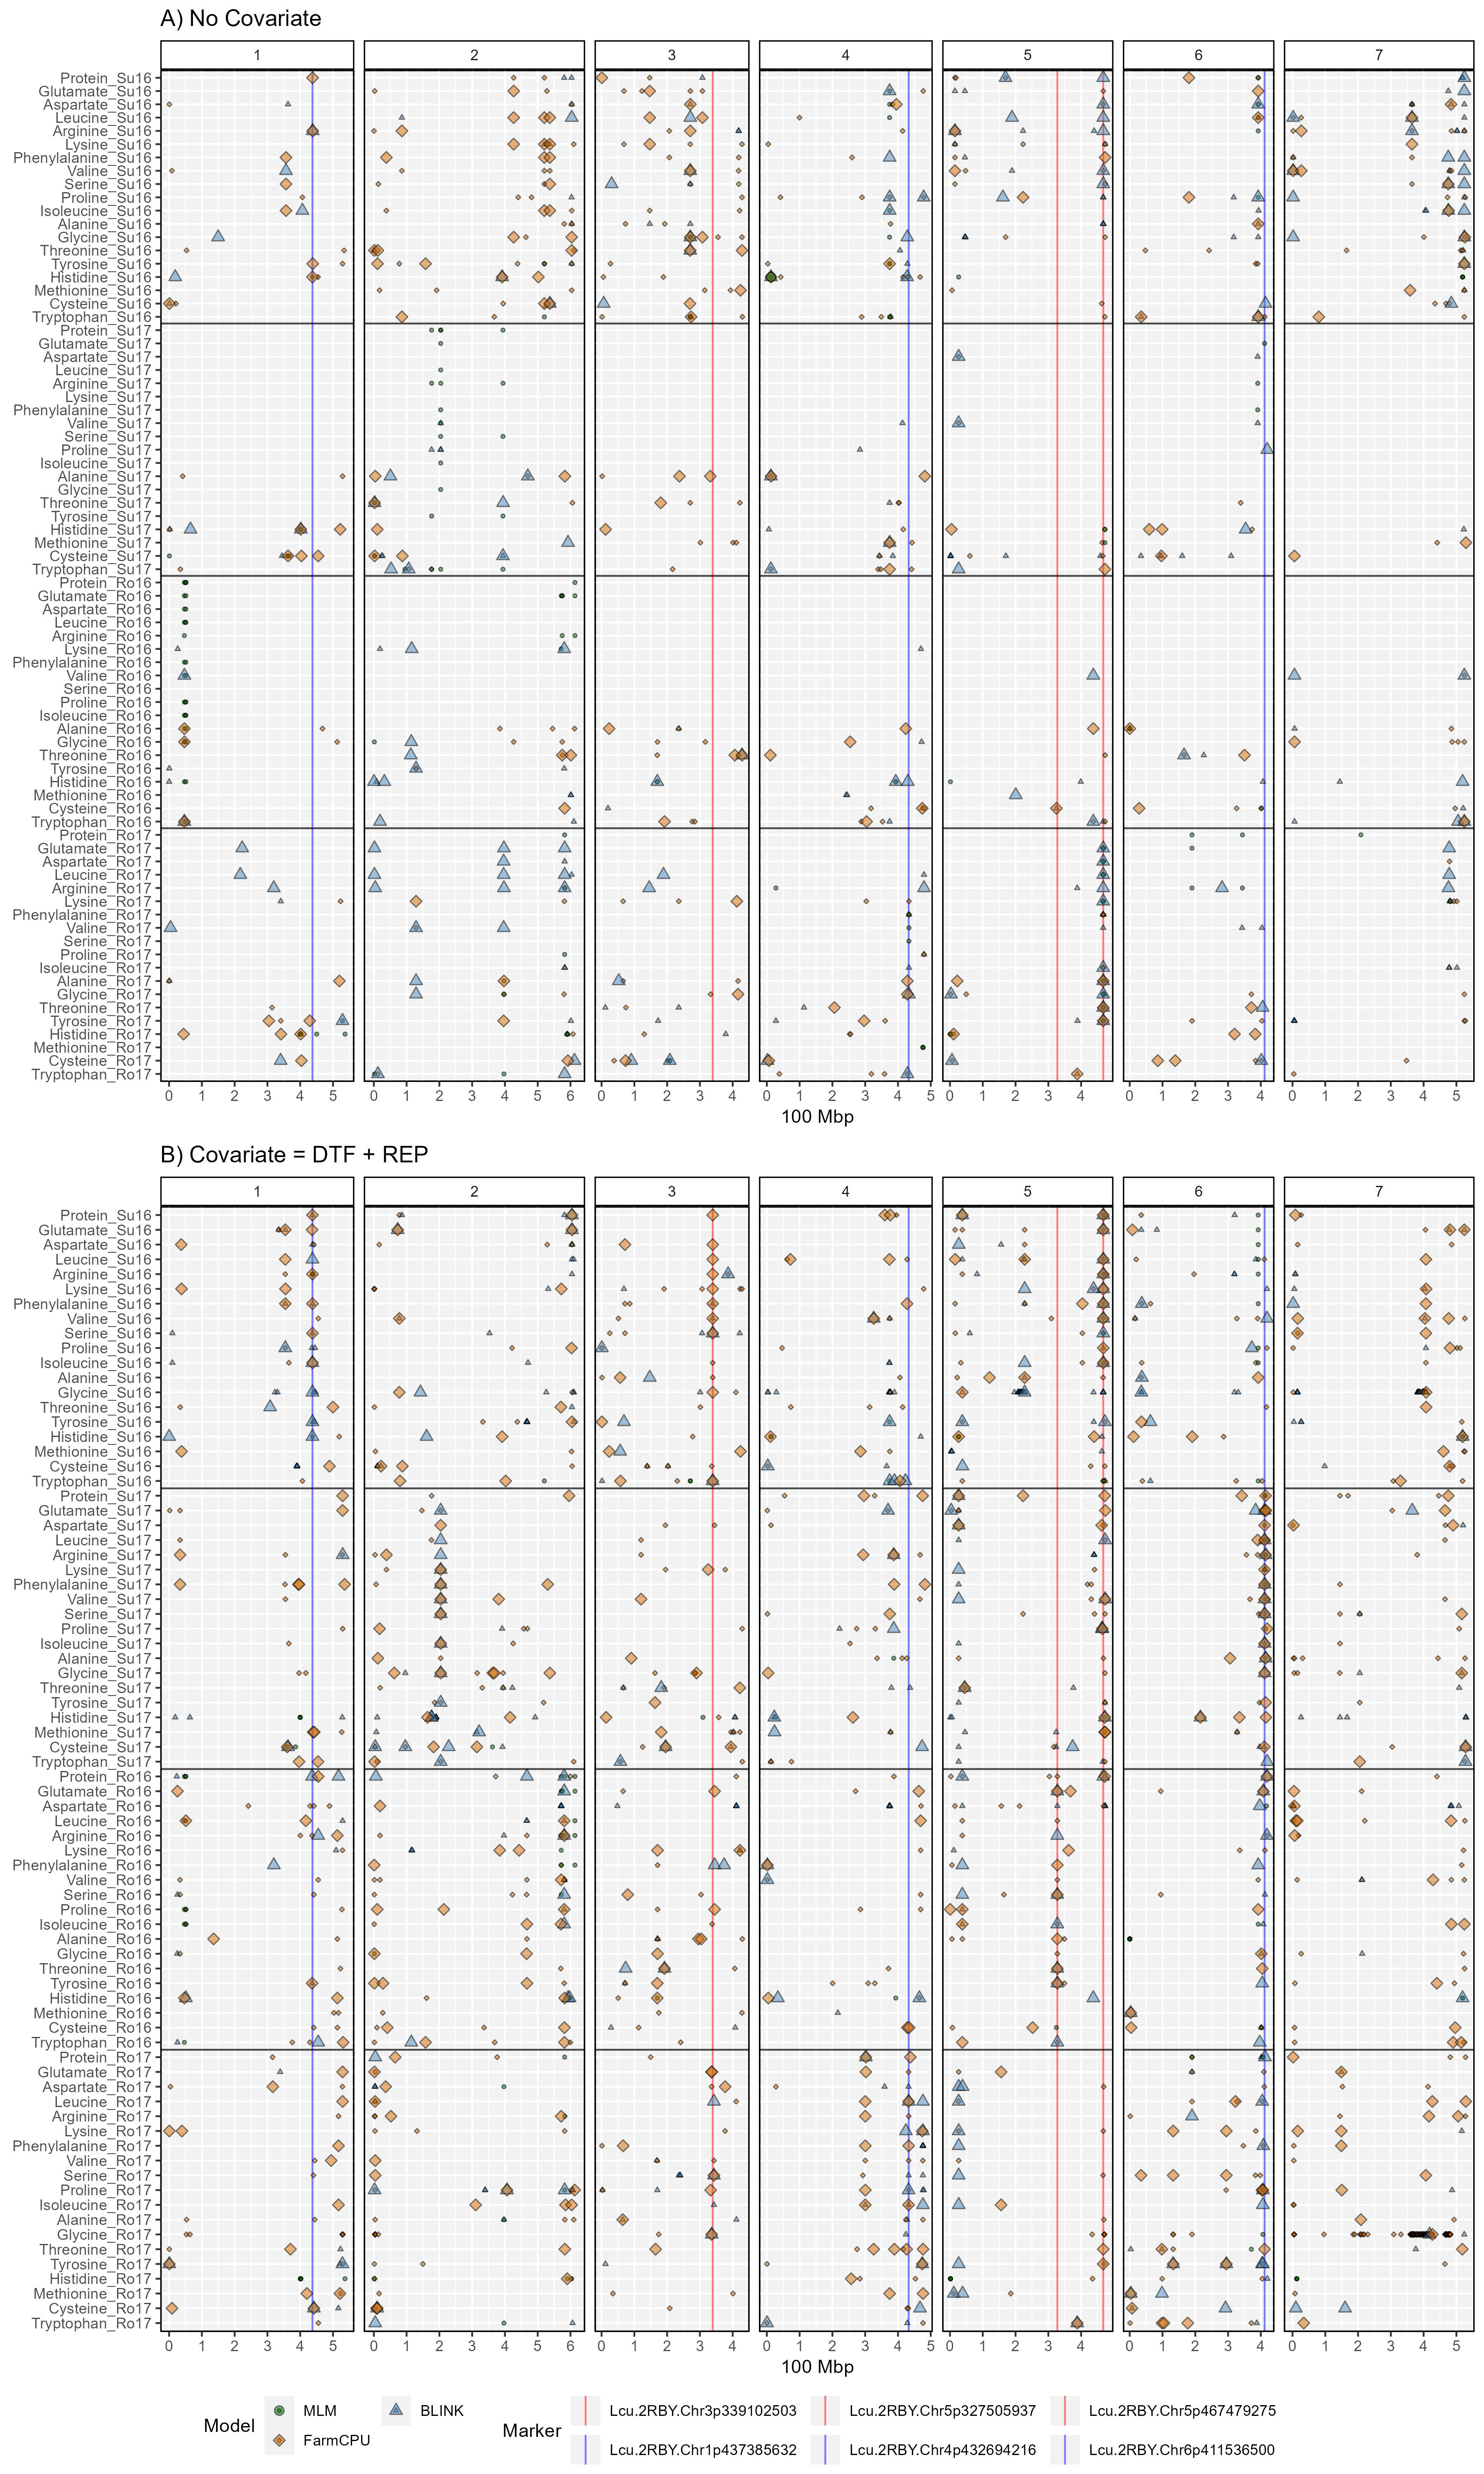
\includegraphics{Figure_04.jpg}

\begin{center}\rule{0.5\linewidth}{0.5pt}\end{center}

\hypertarget{figure-5}{%
\subsection{Figure 5}\label{figure-5}}

\includegraphics{Figure_05a.jpg}

\includegraphics{Figure_05b.jpg}

\includegraphics{Figure_05c.jpg}

\includegraphics{Figure_05d.jpg}

\begin{center}\rule{0.5\linewidth}{0.5pt}\end{center}

\hypertarget{supplemental-figures}{%
\section{Supplemental Figures}\label{supplemental-figures}}

\hypertarget{supplemental-figure-1}{%
\subsection{Supplemental Figure 1}\label{supplemental-figure-1}}

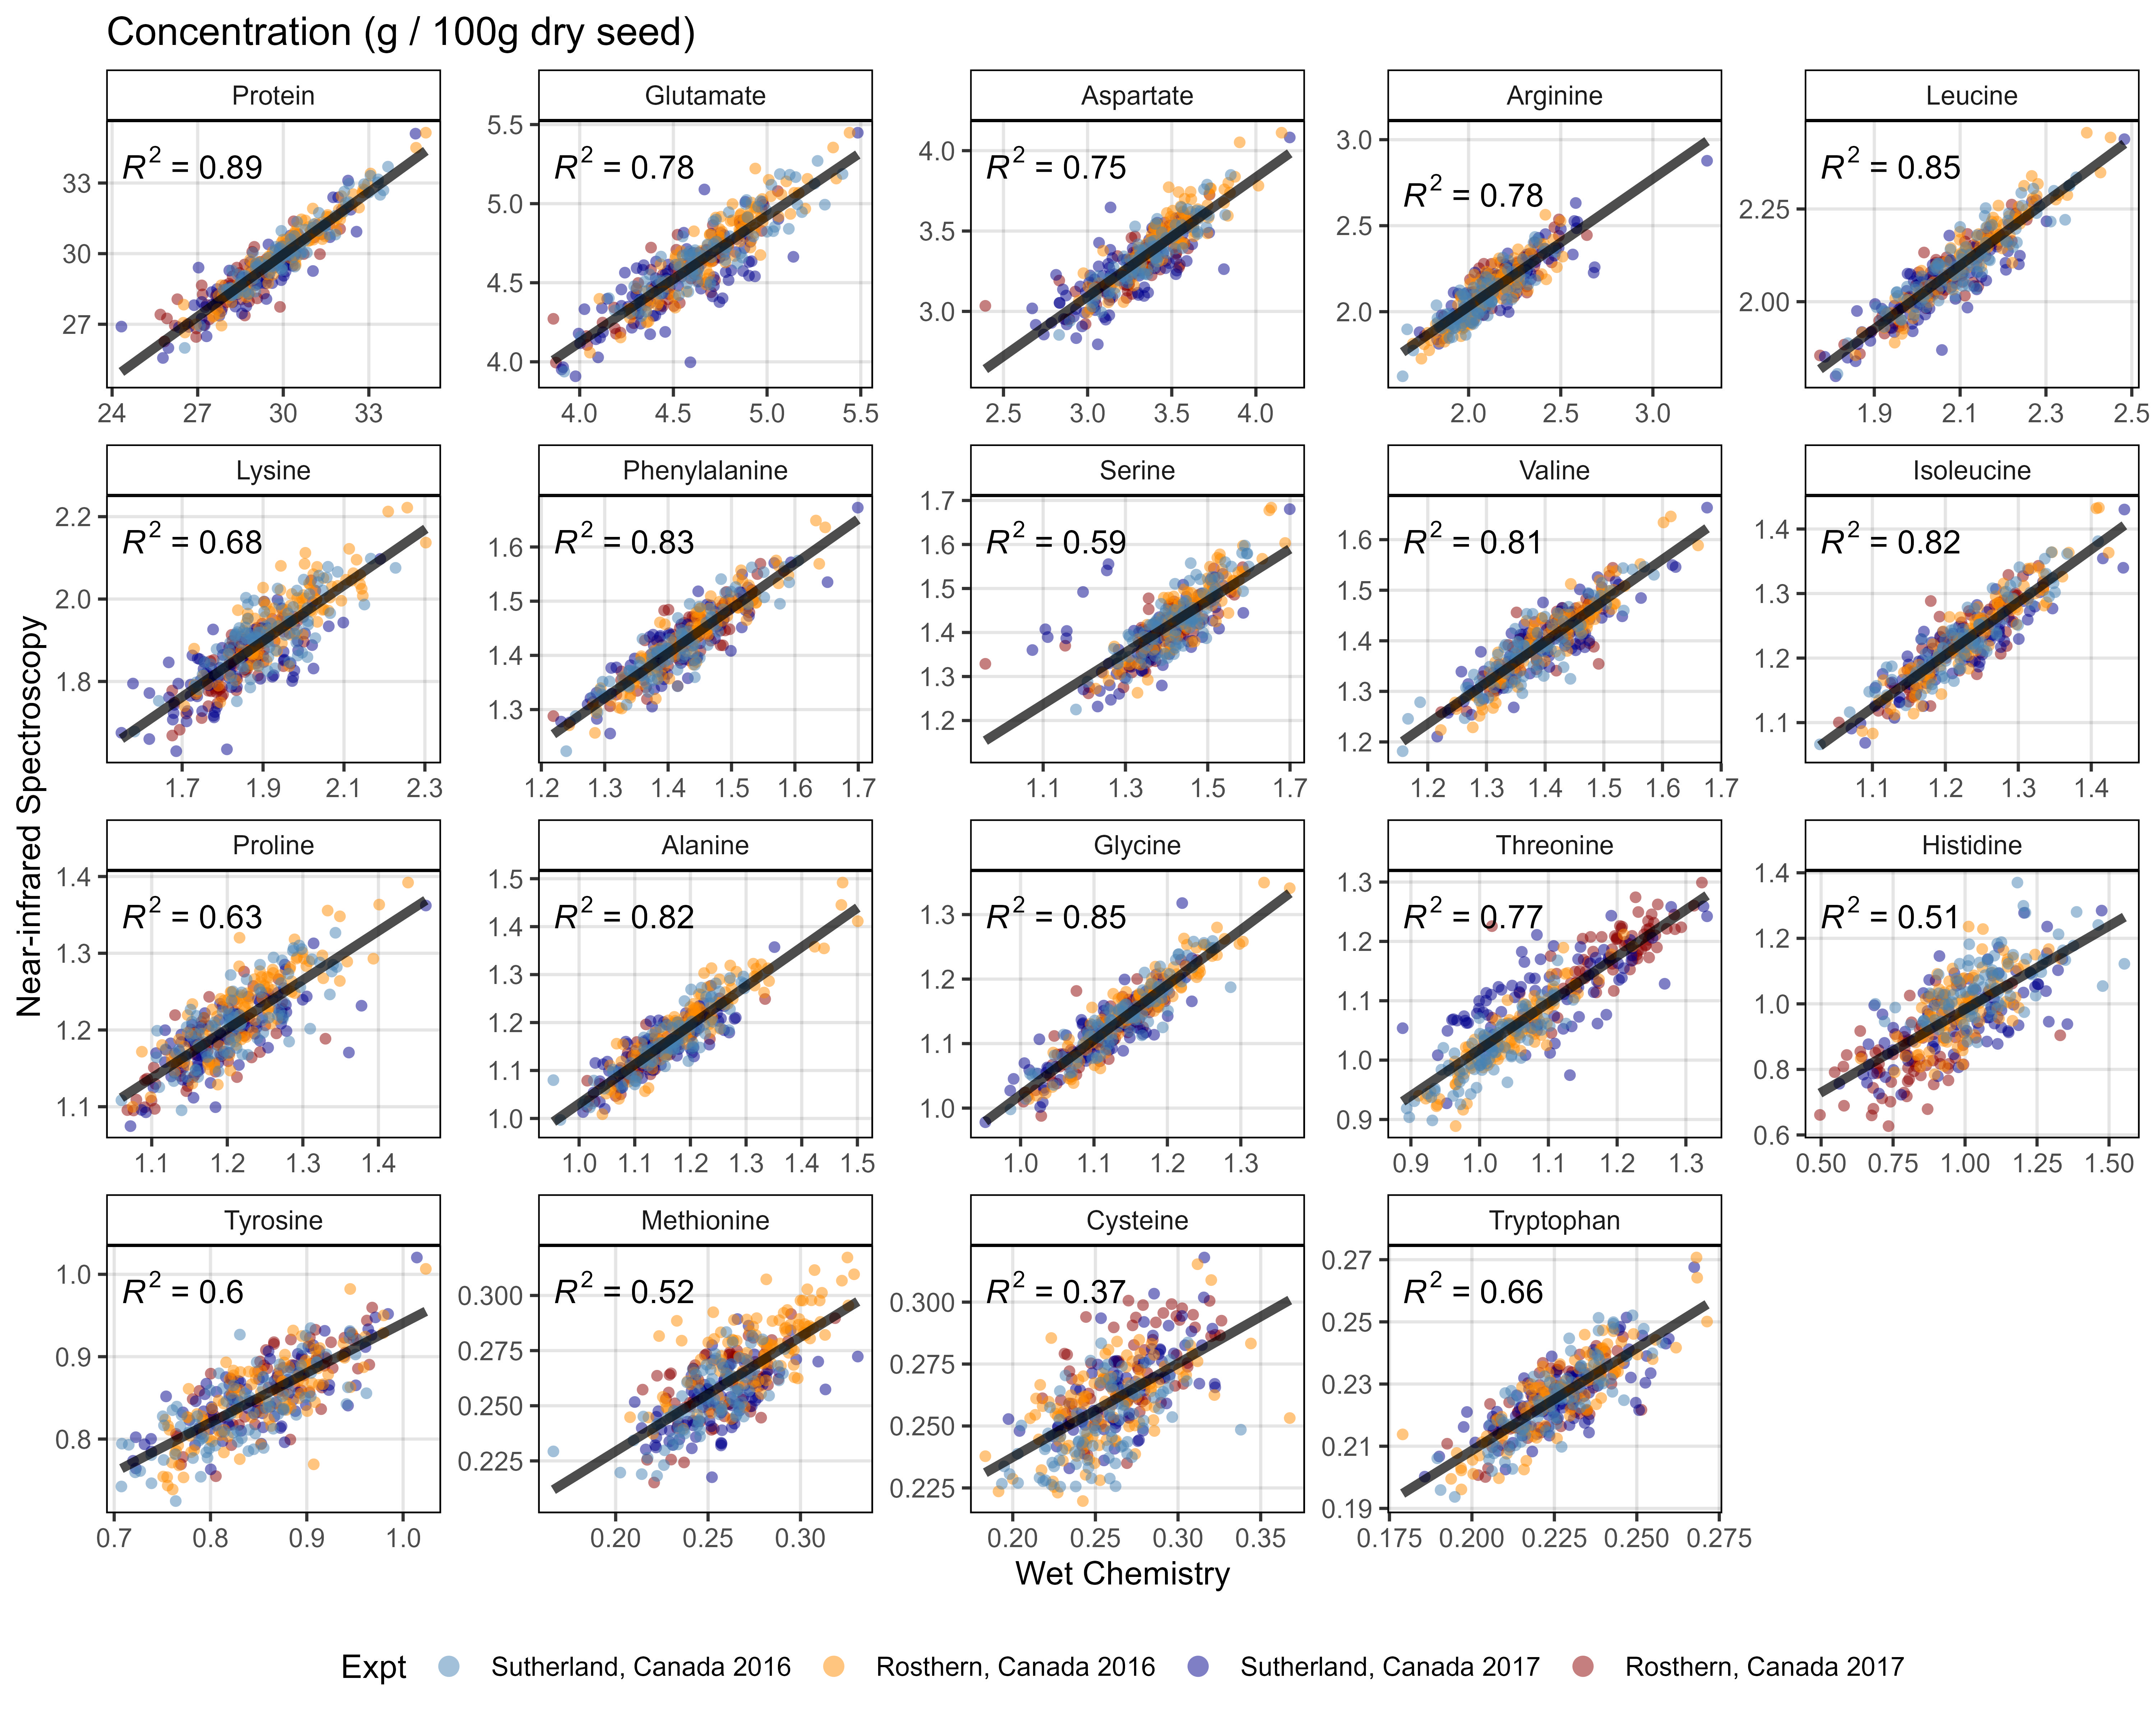
\includegraphics{Supplemental_Figure_01.jpg}

\begin{center}\rule{0.5\linewidth}{0.5pt}\end{center}

\hypertarget{supplemental-figure-2}{%
\subsection{Supplemental Figure 2}\label{supplemental-figure-2}}

\includegraphics{Supplemental_Figure_02.jpg}

\begin{center}\rule{0.5\linewidth}{0.5pt}\end{center}

\hypertarget{supplemental-figure-3}{%
\subsection{Supplemental Figure 3}\label{supplemental-figure-3}}

\includegraphics{Supplemental_Figure_03.jpg}

\begin{center}\rule{0.5\linewidth}{0.5pt}\end{center}

\hypertarget{supplemental-figure-4}{%
\subsection{Supplemental Figure 4}\label{supplemental-figure-4}}

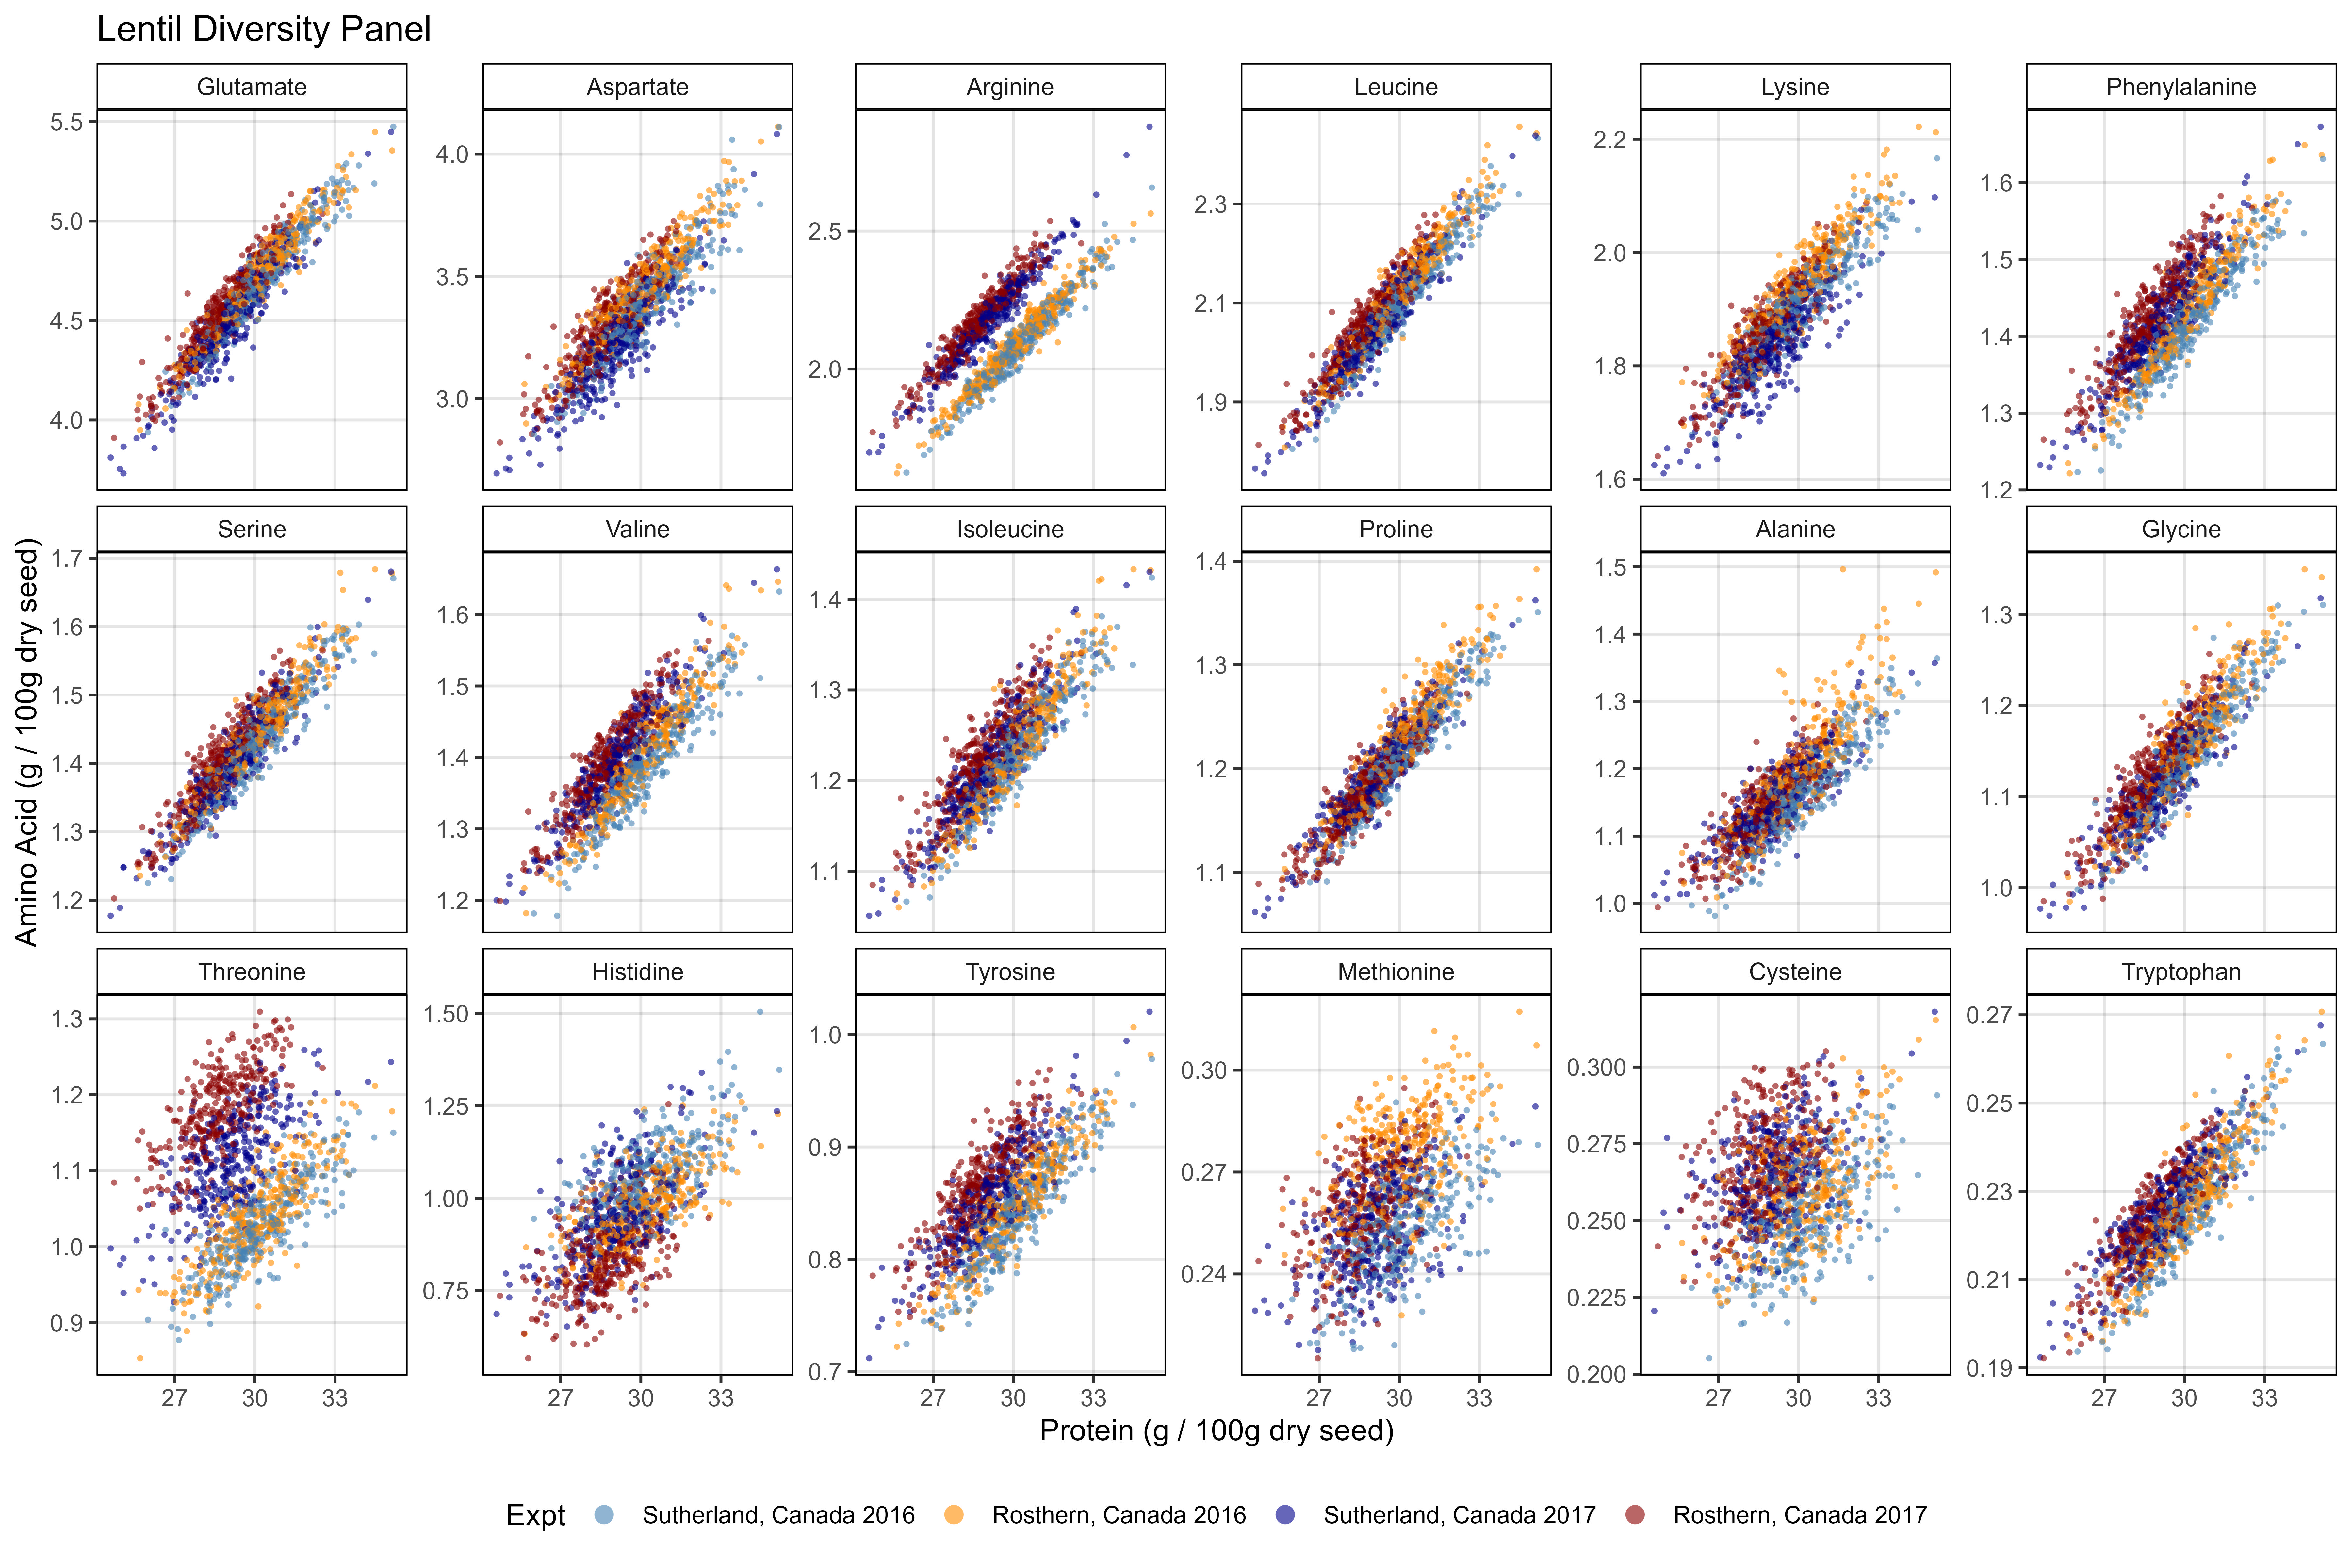
\includegraphics{Supplemental_Figure_04.jpg}

\begin{center}\rule{0.5\linewidth}{0.5pt}\end{center}

\hypertarget{supplemental-figure-5}{%
\subsection{Supplemental Figure 5}\label{supplemental-figure-5}}

\includegraphics{Supplemental_Figure_05a.jpg}

\includegraphics{Supplemental_Figure_05b.jpg}

\includegraphics{Supplemental_Figure_05c.jpg}

\includegraphics{Supplemental_Figure_05d.jpg}

\begin{center}\rule{0.5\linewidth}{0.5pt}\end{center}

\hypertarget{additional-figures}{%
\section{Additional Figures}\label{additional-figures}}

\hypertarget{additional-figure-1}{%
\subsection{Additional Figure 1}\label{additional-figure-1}}

\includegraphics{Additional/Additional_Figure_01.jpg}

\begin{center}\rule{0.5\linewidth}{0.5pt}\end{center}

\hypertarget{additional-figure-2}{%
\subsection{Additional Figure 2}\label{additional-figure-2}}

\includegraphics{Additional/Additional_Figure_02.jpg}

\begin{center}\rule{0.5\linewidth}{0.5pt}\end{center}

\hypertarget{additional-figure-3}{%
\subsection{Additional Figure 3}\label{additional-figure-3}}

\includegraphics{Additional/Additional_Figure_03.jpg}

\begin{center}\rule{0.5\linewidth}{0.5pt}\end{center}

\hypertarget{additional-figure-4}{%
\subsection{Additional Figure 4}\label{additional-figure-4}}

\includegraphics{Additional/Additional_Figure_04.jpg}

\begin{center}\rule{0.5\linewidth}{0.5pt}\end{center}

\hypertarget{additional-figure-5}{%
\subsection{Additional Figure 5}\label{additional-figure-5}}

\includegraphics{Additional/Additional_Figure_05.jpg}

\begin{center}\rule{0.5\linewidth}{0.5pt}\end{center}

\hypertarget{additional-figure-6}{%
\subsection{Additional Figure 6}\label{additional-figure-6}}

\includegraphics{Additional/Additional_Figure_06.jpg}

\begin{center}\rule{0.5\linewidth}{0.5pt}\end{center}

\hypertarget{additional-figure-7}{%
\subsection{Additional Figure 7}\label{additional-figure-7}}

\includegraphics{Additional/Additional_Figure_07.jpg}

\begin{center}\rule{0.5\linewidth}{0.5pt}\end{center}

© Derek Michael Wright

\end{document}
